\documentclass[10pt]{amsart}
\usepackage[margin=1.4in]{geometry}
\usepackage{amssymb,amsmath,enumitem,url}
\usepackage{graphicx,subfig}
\graphicspath{ {./images/} }

\newcommand{\D}{\mathrm{d}}
\newcommand{\I}{\mathrm{i}}
\DeclareMathOperator{\E}{e}
\DeclareMathOperator{\OO}{O}
\DeclareMathOperator{\oo}{o}
\DeclareMathOperator{\erfc}{erfc}
\DeclareMathOperator{\real}{Re}
\DeclareMathOperator{\imag}{Im}
\usepackage{tikz}
\usepackage[framemethod=tikz]{mdframed}
\theoremstyle{nonumberplain}

\mdtheorem[innertopmargin=-5pt]{sol}{Solution}
%\newmdtheoremenv[innertopmargin=-5pt]{sol}{Solution}

\begin{document}
\pagestyle{empty}

\newcommand{\mline}{\vspace{.2in}\hrule\vspace{.2in}}


\title{\bf { AMATH 567 Fall 2024 \\ Homework 1 ---
    Due Sept. 30 on Gradescope by 1:30pm\\
  The 48 hour late penalty is waived for this assignment} }


\maketitle

\begin{center}
  All solutions must include significant justification to receive full credit.  If you handwrite your assignment you must either do so digitally or if it is written on paper you must \emph{scan} your work.  A standard photo is not sufficient.  \vskip 4pt

  If you work with others on the homework, you must name your collaborators.
\end{center}


\mline
\begin{enumerate}[label={\bf {\arabic*}:}]
\item  From A\&F: 1.1.1: (b, e)
Express each of the following complex numbers in exponential form: \\
b) $-i$
\textit{Solution:}
\begin{eqnarray*}
-i &=& 0 -i \\
   &=& 0 + i(-1) \\
   &=& \cos(\frac{3\pi}{2}) + i \sin(\frac{3\pi}{2}) \\
   &=& e^{i\frac{3\pi}{2}}
\end{eqnarray*}
\qed \\
e) $\frac{1}{2}-\frac{\sqrt{3}}{2}i$
\textit{Solution:}
\begin{eqnarray*}
\frac{1}{2} - \frac{\sqrt{3}}{2}i &=& \cos(\frac{5\pi}{3}) + i \sin(\frac{5\pi}{3}) \\
					    &=& e^{i\frac{5\pi}{3}}
\end{eqnarray*}
\qed \\

\item From A\&F: 1.1.2: (b, c, d)
Express each of the following in the form $a + bi$, where $a$ and $b$ are real \\
b) $\frac{1}{1 + i}$
\textit{Solution:}
\begin{eqnarray*}
\frac{1}{1 + i} &=& \frac{1}{1 + i} \frac{(1 - i)}{(1 - i)} \\
		     &=& \frac{1 - i}{1 + i - i - i^2} \\
		     &=& \frac{1 - i}{1 + 1} \\
		     &=& \frac{1 - i}{2} \\
		     &=& \frac{1}{2} - \frac{1}{2}i
\end{eqnarray*}
\qed \\
c) $(1 + i)^3$
\textit{Solution:}
\begin{eqnarray*}
(1 + i)^3 &=& (1 + i)(1 + i)(1 + i) \\
              &=& (1 + i + i + i^2)(1 + i) \\ 
              &=& (1 + 2i - 1)(1 + i) \\
              &=& 2i(1 + i) \\
              &=& 2i + 2i^2 \\
              &=& 2i - 2 \\
              &=& -2 + 2i
\end{eqnarray*}
\qed \\
d) $|3 + 4i|$
\textit{Solution:}
\begin{eqnarray*}
|3 + 4i| &=& \sqrt{3^2 + 4^2} \\
              &=& \sqrt{9 + 16} \\ 
              &=& \sqrt{25} \\
              &=& 5 \\
              &=& 5 + 0i
\end{eqnarray*}
\qed \\


\item From A\&F: 1.1.3: (d)  Solve for the roots of the following equations \\
d) $z^4 + 2z^2 + 2 = 0$ \textit{Solution:} \\
We begin by making a substitution $z^2 = x$ giving us a simpler quadratic equation $x^2 + 2x + 2 = 0$ which we apply the quadratic formula to obtain
\begin{eqnarray*}
x &=& \frac{-2 \pm \sqrt{4 - 8}}{2} \\
   &=& \frac{-2 \pm \sqrt{-4}}{2} \\
   &=& \frac{-2 \pm 2i}{2} \\
   &=& -1 \pm i \quad \text{thus} \\
x &=& -1 + i, -1 - i. \\
\end{eqnarray*}
Plugging this back into our substitution yields
\begin{eqnarray*}
z^2 &=& x \\
z^2 &=& -1 + i \\
\sqrt{z^2} &=& \sqrt{-1 + i} \\
z &=& \pm \sqrt{-1 + i} \quad \text{and} \\
z &=& \pm \sqrt{-1 - i} \quad \text{where $x = -1 - i$}.
\end{eqnarray*}
We don't stop here, but further convert these complex solutions into polar form $x + iy = \rho(cos(\theta) + i\sin(\theta))$ where $\rho = \sqrt{x^2 + y^2}$ as follows. 
Let's begin where $z = \pm \sqrt{-1 + i}$.
First, we rewrite $-1 + i$ by calculating $\rho$ and $\theta$ which end up being $\rho = \sqrt{2}$ and $\theta = \frac{3\pi}{4}$. Thus,
\begin{eqnarray*}
\pm \sqrt{-1 + i} &=& \pm (-1 + i)^\frac{1}{2} \\
			&=& \pm (\sqrt{2}(\cos{\frac{3\pi}{4}}) + i\sin{\frac{3\pi}{4}})^\frac{1}{2} \\
			&=& \pm (\sqrt{2}e^{i \frac{3\pi}{4}})^\frac{1}{2} \\
			&=& \pm 2^{\frac{1}{4}}e^{i \frac{3\pi}{8}}.
\end{eqnarray*}
The $z = \pm \sqrt{-1 -i}$ case is similar except when we calculate $\theta$ for the complex number $ -1 -i $ we get $\theta = \frac{5\pi}{4}$.
Therefore, we have
\begin{eqnarray*}
z &=& \pm 2^{\frac{1}{4}}e^{i \frac{3\pi}{8}} \quad \text{and} \\
   &=& \pm 2^{\frac{1}{4}}e^{i \frac{5\pi}{8}}.
\end{eqnarray*}
However, we want to simplify this even more precisely then to leave these roots with the $\pm$ notation.
Recall Euler's Identity, $e^{i\pi} + 1 = 0$, thus $-1 = e^{i\pi}$. We use this substitution in the cases where $\pm$ resolves to $-$ to simplify further:
\begin{eqnarray*}
z &=& -2^{\frac{1}{4}}e^{i \frac{3\pi}{8}} \\
   &=& (-1) 2^{\frac{1}{4}}e^{i \frac{3\pi}{8}} \\
   &=& (e^{i\pi}) 2^{\frac{1}{4}}e^{i \frac{3\pi}{8}} \\
   &=& 2^{\frac{1}{4}}e^{i\pi}e^{i \frac{3\pi}{8}} \\
   &=& 2^{\frac{1}{4}}e^{i\pi + i \frac{3\pi}{8}} \\
   &=& 2^{\frac{1}{4}}e^{i \frac{11\pi}{8}} \quad \text{and} \\
z &=& -2^{\frac{1}{4}}e^{i \frac{5\pi}{8}} = 2^{\frac{1}{4}}e^{i \frac{13\pi}{8}}.
\end{eqnarray*}
In conclusion our final set of roots solving the equation $z^4 + 2z^2 + 2 = 0$ are the following:
$$
z = 2^{\frac{1}{4}}e^{i \frac{3\pi}{8}}, \enspace
2^{\frac{1}{4}}e^{i \frac{5\pi}{8}}, \enspace
2^{\frac{1}{4}}e^{i \frac{11\pi}{8}}, \enspace
2^{\frac{1}{4}}e^{i \frac{13\pi}{8}}.
$$ \\
\qed \\

\item From A\&F: 1.1.4: (d,f)  Establish the following results:\\
d) $\Re(z) \leq |z|$ \textit{Solution:} \\
We start by reminding ourselves of a few definitions. The complex number $z = x +iy$ where $\Re(z) = x$.
Additionally, the absolute value or modulus is defined as $|z| = \sqrt{x^2 + y^2}$.
Therefore, it is equivalent to show that $x \leq \sqrt{x^2 + y^2}$.
Suppose we don't know the relationship between these two quantities, we will show that it must be so.
\begin{eqnarray*}
x &\stackrel{?}{\leq}& \sqrt{x^2 + y^2} \\
x^2 &\stackrel{?}{\leq}& \sqrt{x^2 + y^2}^2 \\
x^2 &\stackrel{?}{\leq}& x^2 + y^2
\end{eqnarray*}
When $y = 0$ this gives us
$$ x^2 = x^2. $$
When $y \neq 0$ then $y^2 > 0$ thus
$$ x^2 < x^2 + y^2.$$
Since, $x^2 \leq x^2 + y^2$, performing the opposite operations of the first few algebraic steps we get $x \leq \sqrt{x^2 + y^2}$.
Which is equivalent to $\Re(z) \leq |z|$ as established at the beginning. \\
\qed \\
f) $|z_1z_2| = |z_1||z_2|$ \textit{Solution:} \\
Define $z_1 = x_1 + iy_1$ and $z_2 = x_2 + iy_2$.
Now time for some fun algebra!
\begin{eqnarray*}
|z_1z_2| &=& |(x_1 + iy_1)(x_2 + iy_2)| \\
	      &=& |x_1x_2 + ix_1y_2 + iy_1x_2 + i^2y_1y_2| \\
	      &=& |(x_1x_2 - y_1y_2) + i(x_1y_2 + y_1x_2)| \\
	      &=& \sqrt{(x_1x_2 - y_1y_2)^2 + (x_1y_2 + y_1x_2)^2} \\
	      &=& \sqrt{x_1^2x_2^2 -2x_1x_2y_1y_2 + y_1^2y_2^2 + x_1^2y_2^2 + 2x_1x_2y_1y_2 + y_1^2x_2^2} \\
	      &=& \sqrt{x_1^2x_2^2  + y_1^2y_2^2 + x_1^2y_2^2 + y_1^2x_2^2} \\
	      &=& \sqrt{(x_1^2 + y_1^2)(x_2^2 + y_2^2)} \\
	      &=& \sqrt{x_1^2 + y_1^2}\sqrt{x_2^2 + y_2^2} \\
	      &=& |z_1||z_2| \\
\end{eqnarray*}
\qed \\

\item For $a, b \in \mathbb C$, define
  \begin{align*}
    a^b = e^{b \log a},
  \end{align*}
  where $a = r e^{i \theta}$, $- \pi < \theta \leq \pi$ and
  \begin{align*}
    \log a = \log r + i \theta,
  \end{align*}
  is the principal branch of the logarithm.  Find the real and
  imaginary parts of
  \begin{align*}
    i^i \quad \text{and} \quad (1 + i)^i.
  \end{align*}
\textit{Solution:} \\
\textbf{Part 1}  $i^i$ \\
Using the first equation we get
$$i^i = e^{i\log{i}}.$$
Before we use the next equation, let's determine $\rho$ and $\theta$ for the complex number $i$.
$$\rho = \sqrt{x^2 + y^2} = \sqrt{0^2 + 1^2} = \sqrt{0 + 1} = \sqrt{1} = 1$$
We need to find $\theta$ s.t.
\begin{eqnarray*}
\rho \cos(\theta) = 1 \cos(\theta) = \cos(\theta) &=& 0 \\
\rho \sin(\theta) = 1 \sin(\theta) = \sin(\theta)  &=& 1
\end{eqnarray*}
therefore $\theta = \frac{\pi}{2}$.
Now combining this information with the provided equation for the principal branch of the logarithm we get
\begin{eqnarray*}
i^i &=& e^{i\log{i}} \\
    &=& e^{i(\log{1}+i\frac{\pi}{2})} \\
    &=& e^{i(\log{1}+i^2\frac{\pi}{2})} \\
    &=& e^{(i\log{1}-\frac{\pi}{2})} \\
    &=& e^{i\log{1}}e^{-\frac{\pi}{2}} \\
    &=& (\cos(\log{1}) + i\sin(\log{1}))e^{-\frac{\pi}{2}} \\
    &=& \frac{\cos(\log{1})}{e^{\frac{\pi}{2}}} + i\frac{\sin(\log{1}))}{e^{\frac{\pi}{2}}} \\
    &=& \frac{\cos(0)}{e^{\frac{\pi}{2}}} + i\frac{\sin(0))}{e^{\frac{\pi}{2}}} \\
    &=& \frac{1}{e^{\frac{\pi}{2}}} + i\frac{0}{e^{\frac{\pi}{2}}} \\
    &=& e^{-\frac{\pi}{2}} + i0 \\
    &=& e^{-\frac{\pi}{2}}.
\end{eqnarray*}
In conclusion, $\Re{(i^i)} = e^{-\frac{\pi}{2}}$ and $\Im{(i^i)} = 0$. \\
\qed \\
\textbf{Part 2} $(1 + i)^i$ \\
Using the first equation we get
$$(1 + i)^i = e^{i\log{(1 + i)}}.$$
Before we use the next equation, let's determine $\rho$ and $\theta$ for the complex number $i$.
$$\rho = \sqrt{x^2 + y^2} = \sqrt{1^2 + 1^2} = \sqrt{1 + 1} = \sqrt{2}$$
We need to find $\theta$ s.t.
\begin{eqnarray*}
\rho \cos(\theta) = \sqrt{2} \cos(\theta) &=& 1 \\
\rho \sin(\theta) = \sqrt{2} \sin(\theta) &=& 1
\end{eqnarray*}
therefore $\theta = \frac{\pi}{4}$.
Now combining this information with the provided equation for the principal branch of the logarithm we get
\begin{eqnarray*}
(1 + i)^i &=& e^{i\log{(1 + i)}} \\
    &=& e^{i(\log{\sqrt{2}}+i\frac{\pi}{4})} \\
    &=& e^{i(\log{\sqrt{2}}+i^2\frac{\pi}{4})} \\
    &=& e^{(i\log{\sqrt{2}}-\frac{\pi}{4})} \\
    &=& e^{i\log{\sqrt{2}}}e^{-\frac{\pi}{4}} \\
    &=& (\cos(\log{\sqrt{2}}) + i\sin(\log{\sqrt{2}}))e^{-\frac{\pi}{4}} \\
    &=& \frac{\cos(\log{\sqrt{2}})}{e^{\frac{\pi}{4}}} + i\frac{\sin(\log{\sqrt{2}}))}{e^{\frac{\pi}{4}}} \\
    &=& \frac{\cos(\frac{1}{2}\log{2})}{e^{\frac{\pi}{4}}} + i\frac{\sin(\frac{1}{2}\log{2}))}{e^{\frac{\pi}{4}}}.
\end{eqnarray*}
In conclusion, $$\Re{((1 + i)^i)} = \frac{\cos(\frac{1}{2}\log{2})}{e^{\frac{\pi}{4}}} \quad \text{and} \quad \Im{((1 + i)^i)} = \frac{\sin(\frac{1}{2}\log{2}))}{e^{\frac{\pi}{4}}}.$$ \qed \\


\item Consider the function $e(z):=\sum_{n=0}^{\infty}
  \frac{z^n}{n!}$, which is defined for all $z \in \mathbb{C}$ (you
  need not show this). Using only the power series, show that
  $e\left(z_1+z_2\right)=e\left(z_1\right) e\left(z_2\right)$. Can you
  find other power series with the same property? \\
\textit{Solution:} \\
Let's start from the left $e\left(z_1+z_2\right)$.
Immediately we will utilize the binomial theorem, $(a + b)^n = \sum_{k=0}^{n} {n \choose k}a^k b^{n-k} $, to rewrite $(z_1+z_2)^n$. \\
\begin{eqnarray*}
e\left(z_1+z_2\right) &=& \sum_{n=0}^{\infty} \frac{(z_1+z_2)^n}{n!} \\
			       &=& \sum_{n=0}^{\infty} \frac{1}{n!} \sum_{k=0}^{n} {n \choose k}z_1^k z_2^{n-k} \\
			       &=& \sum_{n=0}^{\infty} \frac{1}{n!} \sum_{k=0}^{n} \frac{n!}{(n-k)! k!}z_1^k z_2^{n-k} \\
			       &=& \sum_{n=0}^{\infty} \frac{n!}{n!} \sum_{k=0}^{n} \frac{z_2^{n-k}}{(n-k)!} \frac{z_1^k}{k!} \\
			       &=& \sum_{n=0}^{\infty} \sum_{k=0}^{n} \frac{z_2^{n-k}}{(n-k)!} \frac{z_1^k}{k!} \\
\end{eqnarray*}
Now, let's start from the right and see if we can get it in the same form.
\begin{eqnarray*}
e\left(z_1\right) e\left(z_2\right) &=& \sum_{n=0}^{\infty} \frac{(z_1)^n}{n!} \sum_{m=0}^{\infty} \frac{(z_2)^m}{m!} \\
			       		        &=& \sum_{n=0}^{\infty} \sum_{m=0}^{\infty} \frac{(z_1)^n}{n!} \frac{(z_2)^m}{m!}
\end{eqnarray*}
We have to try and rewrite the sum a little to look more like the binomial version we arrived at from the left.
In order to talk through this we will draw a picture.
\begin{figure}[h]
  \subfloat[The lattice of terms being summed in the $m$ direction followed by the $n$ direction.]{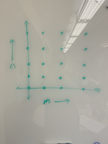
\includegraphics[width=0.4\textwidth]{lattice1}\label{fig:f1}} \quad \quad
  \subfloat[The lattice of terms being summed along the diagonals]{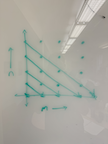
\includegraphics[width=0.4\textwidth]{lattice2}\label{fig:f2}}
  \caption{We use these lattices to demonstrate the change of indices in the summation in the second half of problem 6.}
\end{figure}
As depicted in Figure \ref{fig:f1}, the double infinite sum of the product of these two polynomials can be represented by a lattice.
Each point represents one element in the sum where the $m$ index is increasing along the typical $x$-axis while the $n$ index is increasing along the typical $y$-axis.
What we want to do is change our summing indices from summing all $m$ terms from $0$ to $\infty$ before incrementing the $n$ index to summing over every term in $j^\text{th}$ diagonal.
Therefore we get the following sum
$$\sum_{j=0}^{\infty} \sum_{\ell = 0}^{j} L_{j-\ell, \ell}$$
where $j$ represents which diagonal we are on and $l$ represents which index along $j^{\text{th}}$ diagonal and $L_{j-\ell, \ell}$ is the corresponding entry from the lattice $L$.
Notice the $j-\ell$ in the lattice index is equivalent to the $m$ index.
Now we rewrite the lattice term as the actual entries from the cross product of the two polynomials
$$\sum_{j=0}^{\infty} \sum_{\ell = 0}^{j} L_{j-\ell, \ell} = \sum_{j=0}^{\infty} \sum_{\ell = 0}^{j} \frac{z_2^{j-\ell}}{(j - \ell)!} \frac{z_1^{\ell}}{\ell!}. $$
To arrive here we have basically just made the substitutions $n = j$ and $m = j - \ell$.
Since this has turned out be in the same form as when we started from the left direction the two are equivalent.
Therefore
$$ e\left(z_1+z_2\right)=e\left(z_1\right) e\left(z_2\right) $$
Additionally we are asked if there are any other power series which satisfy this property.
To begin we will define a new function $f(z_1 + z_2) = \sum_{n=0}^\infty a_n\frac{(z_1 + z_2)^n}{n!}.$
Following the same logic as our first argument in this problem, we can write this as 
\begin{eqnarray*}
f(z_1 + z_2) = \sum_{n=0}^\infty a_n\frac{(z_1 + z_2)^n}{n!} &=& \sum_{n=0}^{\infty} \frac{a_n}{n!} \sum_{k=0}^{n} {n \choose k}z_1^k z_2^{n-k} \\
											   &=& \sum_{n=0}^{\infty} \frac{a_n}{n!} \sum_{k=0}^{n} \frac{n!}{(n-k)! k!}z_1^k z_2^{n-k} \\
											   &=& \sum_{n=0}^{\infty} \frac{n!}{n!} \sum_{k=0}^{n} \frac{a_n}{(n-k)! k!}z_1^k z_2^{n-k} \\
											   &=& \sum_{n=0}^{\infty} \sum_{k=0}^{n} a_n\frac{z_2^{n-k}}{(n-k)!}\frac{z_1^k}{ k!} \\
											   &=& \sum_{n=0}^{\infty} \sum_{m=0}^{\infty} a_n\frac{z_2^m}{m!}\frac{z_1^n}{ n!} \\
											   &=& \sum_{n=0}^{\infty} \frac{z_1^n}{ n!}\sum_{m=0}^{\infty} a_n\frac{z_2^m}{m!} \\
											   &=& \text{TBD}
\end{eqnarray*}
\qed
  
\item Consider the complex-valued expression
$$
f(z)=z^{1 / 2}
$$
where $z=x+i y$, with $x, y \in \mathbb{R}$. Derive explicit
expressions for the real and imaginary part(s) of $f(z)$ in terms of
$x$ and $y$. If you make any choices (e.g. for branch cuts), show how
they impact your answer. Your answer should not contain any trig
functions.\\
\textit{Solution:} \\
First, note the following once again
\begin{eqnarray*}
z &=& x +iy \\
x &=& \rho \sin(\theta) \\
y &=& \rho \cos(\theta)
\end{eqnarray*}
Applying these to $f(z)=z^{1 / 2}$ we see
\begin{eqnarray*}
f(z) &=& z^{1 / 2} \\
      &=& (\rho \cos \theta + i \rho \sin \theta)^{1 / 2} \\
      &=& \sqrt{\rho}(\cos \theta + i \sin \theta)^{1 / 2} \\
      &=& \sqrt{\rho}(e^{i \pi})^{1 / 2} \\
      &=& \sqrt{\rho}e^\frac{i \pi}{2} \\
      &=& \sqrt{\rho}\left(\cos \frac{\theta}{2} +i \sin\frac{\theta}{2}\right). \\
\end{eqnarray*}
We need to remind ourselves of the following half angle trig identities
$$ \cos \frac{\theta}{2} = \text{sgn} \left(\cos \frac{\theta}{2}\right) \sqrt{ \frac{ 1 + \cos \theta }{ 2 }} $$
$$ \sin \frac{\theta}{2} = \text{sgn} \left(\sin \frac{\theta}{2}\right) \sqrt{ \frac{ 1 - \cos \theta }{ 2 }}. $$
Before we make these substitutions let's actualize the value of their signs by liming the range of values that $\theta$ can take on.
Let's limit it such that $\theta \in [0, \pi]$, then $\text{sgn} \left(\cos \frac{\theta}{2}\right)$ and $\text{sgn} \left(\cos \frac{\theta}{2}\right)$ are both positive.
Continuing where we left off earlier, we plug in these half angle identities
\begin{eqnarray*}
\sqrt{\rho}\left(\cos \frac{\theta}{2} +i \sin\frac{\theta}{2}\right) &=& \sqrt{\rho}\left(\sqrt{ \frac{ 1 + \cos \theta }{ 2 }} +i \sqrt{ \frac{ 1 - \cos \theta }{ 2 }}\right) \\
      &=& \sqrt{ \frac{ \rho + \rho \cos \theta }{ 2 }} +i \sqrt{ \frac{ \rho - \rho \cos \theta }{ 2 }} \\
      &=& \sqrt{ \frac{ \sqrt{x^2 + y^2} + x }{ 2 }} +i \sqrt{ \frac{ \sqrt{x^2 + y^2} - x }{ 2 }}
\end{eqnarray*}
therefore, we have $$\Re{f(z)} = \sqrt{ \frac{ \sqrt{x^2 + y^2} + x }{ 2 }}$$ and $$\Im{(f(z)} = \sqrt{ \frac{ \sqrt{x^2 + y^2} - x }{ 2 }}.$$
On the other hand, if we had chosen to limit $\theta$ to the other half of the unit circle such that $\theta \in [\pi, 2\pi]$, then $\text{sgn} \left(\cos \frac{\theta}{2}\right)$ would now be negative and $\text{sgn} \left(\cos \frac{\theta}{2}\right)$ would still be positive.
This small difference would result in only a sign change for the substituted term which would carry through to the end resulting in the following solution
$$f(z) = -\sqrt{ \frac{ \sqrt{x^2 + y^2} + x }{ 2 }} +i \sqrt{ \frac{ \sqrt{x^2 + y^2} - x }{ 2 }}$$
therefore, in this case we have $$\Re{f(z)} = -\sqrt{ \frac{ \sqrt{x^2 + y^2} + x }{ 2 }}$$ and $$\Im{(f(z)} = \sqrt{ \frac{ \sqrt{x^2 + y^2} - x }{ 2 }}.$$
\qed


\item (Solution of the cubic) Consider the cubic equation

$$
x^3+a x^2+b x+c=0,
$$

where $a, b$ and $c$ are given numbers.
\begin{itemize}
\item Use the change of variables $x=y-a / 3$ to reduce the equation to the form

$$
y^3+p y+q=0
$$

Find expressions for $p$ and $q$. \\
\textit{Solution:} \\
$$\left(y - \frac{a}{3}\right)^3 + a\left(y - \frac{a}{3}\right)^2 + b\left(y - \frac{a}{3}\right) + c $$
\begin{eqnarray*}
&=& \left(y^2 - \frac{2a}{3}y + \frac{a^2}{9}\right)\left(y - \frac{a}{3}\right) + a\left(y^2 - \frac{2a}{3}y + \frac{a^2}{9}\right) + by - \frac{ba}{3} + c \\
&=& y^3 - ay^2 + \frac{1}{3}a^2 y - \frac{a^3}{27} + ay^2 - \frac{2a^2}{3}y + \frac{a^3}{9} + by - \frac{ba}{3} + c \\
&=& y^3 + \frac{1}{3}a^2 y - \frac{a^3}{27} - \frac{2a^2}{3}y + \frac{a^3}{9} + by - \frac{ba}{3} + c \\
&=& y^3 + \frac{1}{3}a^2 y  - \frac{2a^2}{3}y + by - \frac{a^3}{27} + \frac{a^3}{9} - \frac{ba}{3} + c \\
&=& y^3 + \left(\frac{1}{3}a^2  - \frac{2a^2}{3} + b\right)y + \left( - \frac{a^3}{27} + \frac{3a^3}{27} - \frac{ba}{3} + c\right)
\end{eqnarray*}
thus $p$ and $q$ are defined as follows $$p = -\frac{1}{3}a^2 + b$$ $$q = \frac{2a^3}{27} - \frac{ba}{3} + c.$$
\item Let $y=u+v$. We're replacing one unknown with two, so we get to impose another constraint later. Check that

$$
u^3+v^3+(3 u v+p)(u+v)+q=0 \text {. }
$$
\textit{Solution:} \\
Let's plug this substitution, $y=u+v$, into our last equation $y^3+p y+q=0$
\begin{eqnarray*}
0 &=& y^3+p y+q \\
   &=& (u + v)^3 + p(u + v) + q \\
   &=& u^3 + 3u^2v + 3uv^2 + v^3 + up + vp + q \\
   &=& u^3 + v^3 + 3u^2v + 3uv^2 + up + vp + q \\
   &=& u^3 + v^3 + (3uv +  p)(u + v) + q.
\end{eqnarray*}

\item Now we impose $3 u v+p=0$, so that

$$
u^3 v^3=-p^3 / 27
$$

Also, from above, we have

$$
u^3+v^3=-q .
$$

Find a quadratic equation satisfied by both $u^3$ and $v^3$. \\
\textit{Solution:} \\
We manipulate the above to get
\begin{eqnarray*}
u^3+v^3&=&-q \\
u^3&=&-q - v^3.
\end{eqnarray*}
Now plugging this in to $u^3 v^3=-p^3 / 27$ we quickly arrive at our quadratic satisfied by either $v^3$ or $u^3$
\begin{eqnarray*}
\left(-q - v^3\right) v^3 &=& -p^3 / 27 \\
-qv^3 - v^6 &=& -p^3 / 27 \\
0 &=& v^6 + qv^3 - p^3 / 27.
\end{eqnarray*}
The $u^3$ version of this comes from making an equivalent substitution and the same algebra as above, after solving $u^3+v^3=-q$ for $v^3$ in terms of $u^3$.

\item Solve this quadratic equation, finding expressions for $u$ and $v$. \\
\textit{Solution:} \\
Using the quadratic formula we get
$$u^3 = \frac{-q \pm \sqrt{q^2 + \frac{4p^3}{27}}}{2}.$$
Before we move on let's determine $v^3$ based on what we found $u^3$ to be. Plugging the equation for $u^3$ into $u^3+v^3=-q$
\begin{eqnarray*}
u^3+v^3 &=& -q \\
\frac{-q \pm \sqrt{q^2 + \frac{4p^3}{27}}}{2} + v^3 &=& -q \\
v^3 &=& -q - \left(\frac{-q \pm \sqrt{q^2 + \frac{4p^3}{27}}}{2}\right) \\
v^3 &=& -q + \frac{q \mp \sqrt{q^2 + \frac{4p^3}{27}}}{2} \\
v^3 &=& -\frac{2q}{2} + \frac{q}{2} \mp \frac{\sqrt{q^2 + \frac{4p^3}{27}}}{2} \\
v^3 &=& -\frac{q}{2} \mp \frac{\sqrt{q^2 + \frac{4p^3}{27}}}{2} \\
v^3 &=& \frac{-q \mp \sqrt{q^2 + \frac{4p^3}{27}}}{2}
\end{eqnarray*}
Importantly, notice that the only difference between $u^3$ and $v^3$ is they will have an opposite sign in front of the square root in the numerator.
Therefore we have the expressions for $u$ and $v$ are as follows
$$u = \left(\frac{-q \pm \sqrt{q^2 + \frac{4p^3}{27}}}{2}\right)^{\frac{1}{3}}$$
$$v = \left(\frac{-q \mp \sqrt{q^2 + \frac{4p^3}{27}}}{2}\right)^{\frac{1}{3}}.$$
Since we are taking a cubic root, we are going to have 3 solutions due to the roots of unity. In our case this results in the following
\begin{eqnarray*}
u &=& \left(\frac{-q \pm \sqrt{q^2 + \frac{4p^3}{27}}}{2}\right)^{\frac{1}{3}} \\
   &=& 1^{\frac{1}{3}}\left(\frac{-q \pm \sqrt{q^2 + \frac{4p^3}{27}}}{2}\right)^{\frac{1}{3}} \\
   &=& e^{i\frac{2\pi k}{3}}\left(\frac{-q \pm \sqrt{q^2 + \frac{4p^3}{27}}}{2}\right)^{\frac{1}{3}}, k = 0, 1, 2 \\
\text{Then we also have} \\
v &=& e^{i\frac{2\pi \ell}{3}} \left(\frac{-q \mp \sqrt{q^2 + \frac{4p^3}{27}}}{2}\right)^{\frac{1}{3}}, \ell = 0, 1, 2
\end{eqnarray*}

\item Finally, obtain an expression for $x$. How many different solutions does your expression give rise to? \\
\textit{Solution:} \\
First I will write out the expression for x explicitly:
\begin{eqnarray*}
x &=& y -\frac{a}{3} \\
   &=& u + v -\frac{a}{3} \\
   &=& e^{i\frac{2\pi k}{3}}\left(\frac{-q \pm \sqrt{q^2 + \frac{4p^3}{27}}}{2}\right)^{\frac{1}{3}} +
   e^{i\frac{2\pi \ell}{3}} \left(\frac{-q \mp \sqrt{q^2 + \frac{4p^3}{27}}}{2}\right)^{\frac{1}{3}} -\frac{a}{3}
\end{eqnarray*}
for $k = 0, 1, 2$ and $\ell = 0, 1, 2$.
For the sake of argument, I am going to realize the + and - sign in front of the square root.
Therefore we are looking at 
$$ x = e^{i\frac{2\pi k}{3}}\left(\frac{-q + \sqrt{q^2 + \frac{4p^3}{27}}}{2}\right)^{\frac{1}{3}} + e^{i\frac{2\pi \ell}{3}} \left(\frac{-q - \sqrt{q^2 + \frac{4p^3}{27}}}{2}\right)^{\frac{1}{3}} -\frac{a}{3}.$$
Now since $k$ and $\ell$ can take on 3 values each this seems to imply that this expression gives rise to 9 solutions.
However, I will show that there are actually only 3 possible solutions since there is a particular relationship between $v$ and $u$.
Recall from earlier that we determined $3uv+p=0$.
Let's manipulate this a little
\begin{eqnarray*}
3uv+p &=& 0 \\
3uv &=& -p \\
v &=& -\frac{p}{3u} \\
v &=& -\frac{p}{3\frac{|u|^2}{\bar{u}}} \\
v &=& -\frac{p \bar{u}}{3|u|^2} \\
v &=& C\bar{u}
\end{eqnarray*}
Where the last few steps come from the fact that $u\bar{u} = |u|^2$ as we've established in class.
Since $p = -\frac{1}{3}a^2 + b$ where $a, b \in \mathbb{R}$, then $p \in \mathbb{R}$ as well.
Therefore, we replace $-\frac{p }{3|u|^2}$ with a constant $C$.
Now we see that $v$ is a real scalar multiple of $\bar{u}$.
Therefore the choice of $u$ based on $k$ impacts the value that $v$ must take on.
In fact choosing $k$ for $u$ determines the value of $\ell$ for $v$ such that it satisfies the constraint just discussed.
Therefore if we choose $k=0$ then the roots of unity portion of $u$ will be $e^{i\frac{2\pi 0}{3}} = e^0 = 1$ which the complex conjugate of this is also $1 = e^0 = e^{i\frac{2\pi 0}{3}}$ therefore $\ell$ must also be 0.
Now if $k=1$ then the roots of unity portion of $u$ will be $e^{i\frac{2\pi}{3}} = -\frac{1}{2} + i\frac{\sqrt{3}}{2}$ which the complex conjugate of this is $-\frac{1}{2} - i\frac{\sqrt{3}}{2} = e^{i\frac{4\pi}{3}}$ therefore $\ell$ must be 2.
Similarly when $k=2$ we must have $\ell = 1$.
Therefore, the expression for $x$ gives rise to 3 unique solutions
\begin{eqnarray*}
x &=& \left(\frac{-q + \sqrt{q^2 + \frac{4p^3}{27}}}{2}\right)^{\frac{1}{3}} + \left(\frac{-q - \sqrt{q^2 + \frac{4p^3}{27}}}{2}\right)^{\frac{1}{3}} -\frac{a}{3}, \\
&& e^{i\frac{2\pi}{3}} \left(\frac{-q + \sqrt{q^2 + \frac{4p^3}{27}}}{2}\right)^{\frac{1}{3}} + e^{i\frac{4\pi}{3}} \left(\frac{-q - \sqrt{q^2 + \frac{4p^3}{27}}}{2}\right)^{\frac{1}{3}} -\frac{a}{3}, \\
&& e^{i\frac{4\pi}{3}} \left(\frac{-q + \sqrt{q^2 + \frac{4p^3}{27}}}{2}\right)^{\frac{1}{3}} + e^{i\frac{2\pi}{3}} \left(\frac{-q - \sqrt{q^2 + \frac{4p^3}{27}}}{2}\right)^{\frac{1}{3}} -\frac{a}{3},
\end{eqnarray*}

\item Use your result to solve the cubic $x^3+3 x^2+6 x+8=0$. \\
\textit{Solution:} \\
We first identify the coefficients here are $a=3$, $b=6$, and $c=8$.
Now let's calculate $p$ and $q$
$$p = -\frac{1}{3}a^2 + b = -\frac{1}{3}3^2 + 6 = - 3 + 6 = 3$$
$$q = \frac{2a^3}{27} - \frac{ba}{3} + c  = \frac{2 \cdot 3^3}{27} - \frac{6 \cdot 3}{3} + 8 = 2 - 6 + 8 = 4$$
Starting with $k = 0$ and $\ell = 0$ we plug these into the solutions for $x$ we get
\begin{eqnarray*}
x &=& \left(\frac{-q + \sqrt{q^2 + \frac{4p^3}{27}}}{2}\right)^{\frac{1}{3}} + \left(\frac{-q - \sqrt{q^2 + \frac{4p^3}{27}}}{2}\right)^{\frac{1}{3}} -\frac{a}{3} \\
   &=& \left(\frac{-4 + \sqrt{4^2 + \frac{4 \cdot 3^3}{27}}}{2}\right)^{\frac{1}{3}} + \left(\frac{-4 - \sqrt{4^2 + \frac{4 \cdot 3^3}{27}}}{2}\right)^{\frac{1}{3}} -\frac{3}{3} \\
   &=& \left(\frac{-4 + \sqrt{16 + 4}}{2}\right)^{\frac{1}{3}} + \left(\frac{-4 - \sqrt{16 + 4}}{2}\right)^{\frac{1}{3}} -1 \\
   &=& \left( - 2 + \frac{\sqrt{20}}{2}\right)^{\frac{1}{3}} + \left(- 2 - \frac{\sqrt{20}}{2}\right)^{\frac{1}{3}} -1 \\
   &=& \left( - 2 + \sqrt{5}\right)^{\frac{1}{3}} + \left(- 2 - \sqrt{5}\right)^{\frac{1}{3}} -1
\end{eqnarray*}

Now where $k=1$ and $\ell=2$
\begin{eqnarray*}
x &=& e^{i\frac{2\pi}{3}} \left(\frac{-q + \sqrt{q^2 + \frac{4p^3}{27}}}{2}\right)^{\frac{1}{3}} + e^{i\frac{4\pi}{3}} \left(\frac{-q - \sqrt{q^2 + \frac{4p^3}{27}}}{2}\right)^{\frac{1}{3}} -\frac{a}{3} \\
   &=& e^{i\frac{2\pi}{3}} \left(\frac{-4 + \sqrt{4^2 + \frac{4 \cdot 3^3}{27}}}{2}\right)^{\frac{1}{3}} + e^{i\frac{4\pi}{3}} \left(\frac{-4 - \sqrt{4^2 + \frac{4 \cdot 3^3}{27}}}{2}\right)^{\frac{1}{3}} -\frac{3}{3} \\
   &=& e^{i\frac{2\pi}{3}} \left(\frac{-4 + \sqrt{16 + 4}}{2}\right)^{\frac{1}{3}} + e^{i\frac{4\pi}{3}} \left(\frac{-4 - \sqrt{16 + 4}}{2}\right)^{\frac{1}{3}} -1 \\
   &=& e^{i\frac{2\pi}{3}} \left( - 2 + \frac{\sqrt{20}}{2}\right)^{\frac{1}{3}} + e^{i\frac{4\pi}{3}} \left(- 2 - \frac{\sqrt{20}}{2}\right)^{\frac{1}{3}} -1 \\
   &=& e^{i\frac{2\pi}{3}} \left( - 2 + \sqrt{5}\right)^{\frac{1}{3}} + e^{i\frac{4\pi}{3}} \left(- 2 - \sqrt{5}\right)^{\frac{1}{3}} -1
\end{eqnarray*}

Now where $k=2$ and $\ell=1$
\begin{eqnarray*}
x &=& e^{i\frac{4\pi}{3}} \left(\frac{-q + \sqrt{q^2 + \frac{4p^3}{27}}}{2}\right)^{\frac{1}{3}} + e^{i\frac{2\pi}{3}} \left(\frac{-q - \sqrt{q^2 + \frac{4p^3}{27}}}{2}\right)^{\frac{1}{3}} -\frac{a}{3} \\
   &=& e^{i\frac{4\pi}{3}} \left(\frac{-4 + \sqrt{4^2 + \frac{4 \cdot 3^3}{27}}}{2}\right)^{\frac{1}{3}} + e^{i\frac{2\pi}{3}} \left(\frac{-4 - \sqrt{4^2 + \frac{4 \cdot 3^3}{27}}}{2}\right)^{\frac{1}{3}} -\frac{3}{3} \\
   &=& e^{i\frac{4\pi}{3}} \left(\frac{-4 + \sqrt{16 + 4}}{2}\right)^{\frac{1}{3}} + e^{i\frac{2\pi}{3}} \left(\frac{-4 - \sqrt{16 + 4}}{2}\right)^{\frac{1}{3}} -1 \\
   &=& e^{i\frac{4\pi}{3}} \left( - 2 + \frac{\sqrt{20}}{2}\right)^{\frac{1}{3}} + e^{i\frac{2\pi}{3}} \left(- 2 - \frac{\sqrt{20}}{2}\right)^{\frac{1}{3}} -1 \\
   &=& e^{i\frac{4\pi}{3}} \left( - 2 + \sqrt{5}\right)^{\frac{1}{3}} + e^{i\frac{2\pi}{3}} \left(- 2 - \sqrt{5}\right)^{\frac{1}{3}} -1
\end{eqnarray*}


\item (Bombelli's equation) Use your result to solve the cubic $x^3-15
  x-4=0$, writing your result explicitly in terms of real and
  imaginary parts. \\
\textit{Solution:} \\
We first identify the coefficients here are $a=0$, $b=-15$, and $c=-4$.
Now let's calculate $p$ and $q$
$$p = -\frac{1}{3}a^2 + b = -\frac{1}{3}0^2 -15 = 0 -15 = -15$$
$$q = \frac{2a^3}{27} - \frac{ba}{3} + c = \frac{2 \cdot 0^3}{27} - \frac{-15 \cdot 0}{3} - 4 = 0 + 0 -4 = -4$$
Starting with $k = 0$ and $\ell = 0$ we plug these into the solutions for $x$ we get
\begin{eqnarray*}
x &=& \left(\frac{-q + \sqrt{q^2 + \frac{4p^3}{27}}}{2}\right)^{\frac{1}{3}} + \left(\frac{-q - \sqrt{q^2 + \frac{4p^3}{27}}}{2}\right)^{\frac{1}{3}} -\frac{a}{3} \\
   &=& \left(\frac{4 + \sqrt{(-4)^2 + \frac{4 \cdot (-15)^3}{27}}}{2}\right)^{\frac{1}{3}} + \left(\frac{4 - \sqrt{(-4)^2 + \frac{4 \cdot (-15)^3}{27}}}{2}\right)^{\frac{1}{3}} -\frac{3}{3} \\
   &=& \left(\frac{4 + \sqrt{16 - 500}}{2}\right)^{\frac{1}{3}} + \left(\frac{-4 - \sqrt{16 - 500}}{2}\right)^{\frac{1}{3}} -1 \\
   &=& \left(2 + \frac{\sqrt{-484}}{2}\right)^{\frac{1}{3}} + \left(2 - \frac{\sqrt{-484}}{2}\right)^{\frac{1}{3}} -1 \\
   &=& \left(2 + \frac{i22}{2}\right)^{\frac{1}{3}} + \left(2 - \frac{i22}{2}\right)^{\frac{1}{3}} -1 \\
   &=& \left(2 + i11\right)^{\frac{1}{3}} + \left(2 - i11\right)^{\frac{1}{3}} -1 \\
\end{eqnarray*}

Now where $k=1$ and $\ell=2$
\begin{eqnarray*}
x &=& \text{TBD}
\end{eqnarray*}

Now where $k=2$ and $\ell=1$
\begin{eqnarray*}
x &=& \text{TBD}
\end{eqnarray*}
\qed
  \end{itemize}



\end{enumerate}

\end{document}

%%% Local Variables:
%%% mode: latex
%%% TeX-master: t
%%% End:
